% FORMAT AND PACKAGES
% {
\documentclass[a4paper]{article}
\usepackage{Styles/hcmut}

% DOCUMENT
\begin{document}
% TITLE PAGE
\begin{titlepage}
\begin{center}
ĐẠI HỌC QUỐC GIA THÀNH PHỐ HỒ CHÍ MINH\\
TRƯỜNG ĐẠI HỌC BÁCH KHOA \\
KHOA KHOA HỌC VÀ KỸ THUẬT MÁY TÍNH
\end{center}

\vspace{1cm}

\begin{figure}[h!]
\begin{center}

\includegraphics[width=3cm]{Images/hcmut.png}
\end{center}
\end{figure}

\vspace{1cm}


\begin{center}
\begin{tabular}{c}
\multicolumn{1}{l}{\textbf{{\Large Mô hình hoá toán  học (CO2011)}}}\\
~~\\
\hline
\\
\multicolumn{1}{l}{\textbf{{\Large Báo cáo bài tập lớn}}}\\
\\
\textbf{\textit{{\Large "Two-Dimension Cutting Stock Problem"}}}\\
\\
\hline
\end{tabular}
\end{center}

\vspace{2cm}

\begin{table}[h]
\centering
    \begin{tabular}{rl}
    \hspace{2 cm}\textbf{Giáo viên hướng dẫn}:
    & Lê Hồng Trang, CSE-HCMUT\\

    & \\[5pt]
    \textbf{Sinh viên thực hiện}: &  Nguyễn Phúc Nhân - 2312438 \emph{(L05 - Nhóm 88)} - \textbf{Nhóm trưởng} \\
    & Phan Đức Nhã - 2312410 \emph{(L06 - Nhóm 88)} \\
    & Lê Hoàng Luân - 2311982 \emph{(L06 - Nhóm 88)} \\
    \end{tabular}
\end{table}

\begin{center}
{\footnotesize Thành phố Hồ Chí Minh, Tháng 12 năm 2024}
\end{center}
\end{titlepage}
\pagebreak

\pagebreak

\tableofcontents
\pagebreak

\printunsrtglossary[type={symbols}, title={Danh sách các ký hiệu}]
\printunsrtglossary[type={abbreviations}, title={Danh sách các từ viết tắt}]
\pagebreak
\listoffigures
\listoftables
\pagebreak

\addcontentsline{toc}{section}{\listfigurename}
\addcontentsline{toc}{section}{\listtablename}

% Member list
\section*{Danh sách thành viên và khối lượng công việc}
\addcontentsline{toc}{section}{Danh sách thành viên và khối lượng công việc}
\begin{center}
    \begin{table}[h]
        \centering
        \begin{tabular}{|c|c|c|l|c|}
        
            \hline
            \textbf{No.} & \textbf{Họ và tên} & \textbf{MSSV} & \textbf{Công việc} & \textbf{\% hoàn thành}\\
            \hline 
        
            %%%%%Student 1%%%%%%%%%%
            \multirow{3}{*}{1} & \multirow{3}{*}{Nguyễn Phúc Nhân} & \multirow{3}{*}{2312438} & 
            - Algorithm& \multirow{3}{*}{100\%}\\
             & &  & - Analyze Result&\\
             & &  & - Use cases&\\
             & &  & - Conclusion&\\
             & &  & - Background&\\
            \hline 
        
            %%%%%Student 2%%%%%%%%%%%
            \multirow{3}{*}{2} & \multirow{3}{*}{Phan Đức Nhã} & \multirow{3}{*}{2312410} & 
            - Introduction& \multirow{3}{*}{100\%}\\
             & &  & - Background&\\
             & &  & - Case Study&\\
            \hline
        
            %%%%%Student 3%%%%%%%%%%%
            \multirow{3}{*}{3} & \multirow{3}{*}{Lê Hoàng Luân} & \multirow{3}{*}{2311982} & 
            - Model& \multirow{3}{*}{100\%}\\
             & &  & - Algorithm&\\
             & &  & - Analyze Result&\\
            \hline
            
        \end{tabular}
    \caption{\label{table1}Danh sách thành viên và khối lượng công việc}
    \end{table}
\end{center}


\pagebreak

\section{Giới thiệu}
\subsection{Bài toán Cắt Tấm (Cutting Stock Problem)}

\hspace{0.5cm}Bài toán cắt vật liệu (CSP) là một bài toán tối ưu quen thuộc trong lĩnh vực nghiên cứu vận hành, tập trung vào cách cắt các tấm nguyên liệu lớn thành các mảnh nhỏ hơn nhằm đáp ứng nhu cầu cụ thể và giảm thiểu lãng phí. Bài toán này rất phổ biến trong các ngành công nghiệp như thép, giấy, dệt may, và kính, nơi nguyên liệu thường có kích thước tiêu chuẩn và cần được cắt theo yêu cầu sản xuất. CSP giúp tối ưu hóa việc sử dụng nguyên liệu, giảm chi phí sản xuất và nâng cao hiệu quả vận hành.

Bài toán này được nhà kinh tế học người Nga Leonid Kantorovich lần đầu tiên đề xuất vào năm 1939 \cite{benamor_cutting_2024}. Đến thập niên 1960, Gilmore và Gomory \cite{benamor_cutting_2024} đã giới thiệu kỹ thuật sinh cột (column generation), giúp giải bài toán cắt tấm một chiều hiệu quả hơn bằng cách tạo ra các mẫu cắt dần dần thay vì giải toàn bộ bài toán cùng lúc. Phương pháp này đã tạo nền tảng cho nhiều kỹ thuật hiện đại.

CSP thường được phân loại dựa trên số chiều và sự đa dạng của nguyên liệu và sản phẩm cần cắt. Với độ phức tạp tính toán cao, CSP thuộc loại bài toán NP-hard \cite{IR}, khiến việc tìm lời giải chính xác trở nên không khả thi trong thời gian hợp lý đối với các bài toán lớn. Vì vậy, nhiều thuật toán và phương pháp gần đúng đã được phát triển.

Nhờ tính ứng dụng cao và khả năng tiết kiệm chi phí đáng kể, CSP vẫn là chủ đề nghiên cứu quan trọng. Các phương pháp hiện đại tích hợp các tiến bộ như kỹ thuật sinh cột, nhánh và cận, và cả học máy, đảm bảo ngành công nghiệp liên tục cải thiện hiệu quả và giảm thiểu lãng phí.

\subsection{Bài toán Cắt Tấm Hai Chiều (Two-Dimension Cutting Stock Problem)}

\hspace{0.5cm}Bài toán cắt tấm hai chiều (2DCSP) là một bài toán tối ưu tổ hợp phức tạp, có vai trò quan trọng trong các ngành công nghiệp như sản xuất, hậu cần, và gia công vật liệu. Mục tiêu của 2DCSP là cắt các mảnh nhỏ từ một nguyên liệu lớn hơn, chẳng hạn như tấm hoặc cuộn, đồng thời giảm thiểu lượng vật liệu bị lãng phí. Bài toán này rất phức tạp do phải cân nhắc yếu tố hình học và tối ưu hóa các mẫu cắt, vốn thay đổi tùy theo hình dạng và phương pháp cắt được sử dụng.

Bài toán 2DCSP được phân loại dựa trên loại hình dạng cần cắt, từ các hình dạng đơn giản như hình chữ nhật và hình tròn cho đến các hình dạng phức tạp và không đều. Mỗi loại hình dạng đều mang đến những thách thức riêng trong việc sắp xếp và cắt từ nguyên liệu hiện có.

Hai kỹ thuật cắt chính thường được sử dụng trong 2DCSP là Cắt kiểu guillotine (guillotine cutting) và Cắt không kiểu guillotine (non-guillotine cutting)

\begin{itemize}
    \item Cắt Kiểu Guillotine: Trong phương pháp này, quá trình cắt bị giới hạn bởi các đường cắt thẳng, kéo dài toàn bộ chiều dài hoặc chiều rộng của nguyên liệu. Mỗi đường cắt được thực hiện từ một cạnh của vật liệu đến cạnh đối diện, và các đường cắt này chia nguyên liệu thành các phần nhỏ hơn. Cắt kiểu guillotine đơn giản hóa bài toán bằng cách giảm số lượng mẫu cắt có thể có, nhưng có thể dẫn đến các giải pháp không tối ưu đối với một số cấu hình hình dạng nhất định.
    \begin{figure}[!htp]
        \centering
        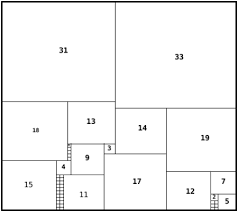
\includegraphics[width=0.25\linewidth]{Images/2dcspgui.png}
        \caption{Minh họa quá trình cắt kiểu Guillotine: Các đường cắt thẳng từ một cạnh đến cạnh đối diện}
        \label{fig:2dcspgui}
    \end{figure}

    \item Cắt Không Kiểu Guillotine: Phương pháp này cho phép linh hoạt hơn trong việc lựa chọn các đường cắt, có nghĩa là cắt có thể thực hiện ở bất kỳ góc độ nào và không bị giới hạn phải cắt qua toàn bộ vật liệu. Mặc dù tính linh hoạt này mang lại cơ hội tối ưu hóa các mẫu cắt hiệu quả hơn, nhưng nó cũng làm tăng độ phức tạp của bài toán, vì có nhiều cấu hình tiềm năng cần xem xét.

    \begin{figure}[!htp]
        \centering
        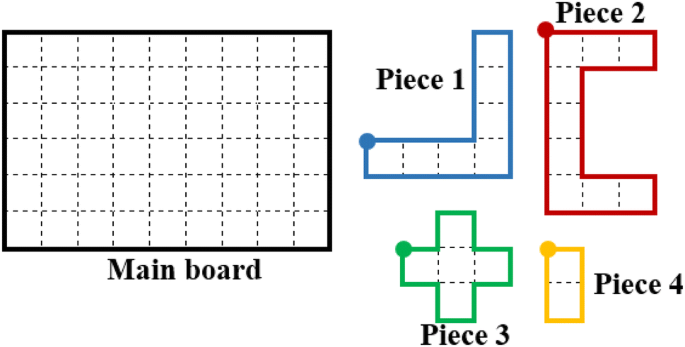
\includegraphics[width=0.5\linewidth]{Images/nongui2dcsp.png}
        \caption{Bài toán cắt tấm hai chiều không kiểu Guillotine}
        \label{fig:enter-label}
    \end{figure}
    
\end{itemize}

Tác động của việc lựa chọn giữa phương pháp cắt kiểu guillotine và không kiểu guillotine là rất lớn. Cắt kiểu guillotine đơn giản hơn khi thực hiện và thường nhanh hơn, nhưng có thể dẫn đến việc lãng phí vật liệu cao đối với các hình dạng không đều hoặc không phải hình chữ nhật. Trong khi đó, cắt không kiểu guillotine cung cấp nhiều cơ hội tối ưu hóa hơn nhưng với cái giá là tăng độ phức tạp tính toán.

Bài toán 2DCSP cũng có ứng dụng rộng rãi trong các tình huống thực tế như sản xuất đồ nội thất, cắt vải, và thậm chí trong thiết kế các bố cục tối ưu cho bảng mạch in (PCBs). Trong tất cả các trường hợp này, mục tiêu vẫn là: giảm thiểu lãng phí và tối đa hóa việc sử dụng nguyên liệu có sẵn, đây là một thách thức quan trọng đòi hỏi việc phát triển các mô hình toán học tinh vi và các thuật toán gần đúng.

\subsection{Cấu trúc bài báo cáo}

\hspace{0.5cm}Nghiên cứu này đóng góp vào bài toán cắt tấm hai chiều (2DCSP) bằng cách giải quyết cả lý thuyết và thực tiễn. Bắt đầu với mô hình toán học ILP, nghiên cứu đánh giá các phương pháp heuristic như Tham lam (Greedy) và Phân bổ Tốt Nhất (Best-Fit), cùng các phương pháp tiên tiến như Tạo Cột (Column Generation). Tính thực tiễn được minh chứng qua nghiên cứu tình huống, áp dụng vào quản lý tài nguyên và cắt bảng mạch in, giúp giảm lãng phí và nâng cao hiệu quả vật liệu. So sánh các thuật toán dựa trên các chỉ số như sử dụng vật liệu và hiệu quả tính toán, nghiên cứu cung cấp cái nhìn về ưu điểm và sự đánh đổi. Cuối cùng, nghiên cứu hướng tới việc tích hợp AI, metaheuristics và ứng dụng trong các lĩnh vực mới như sản xuất gia công bổ sung và hậu cần, đóng góp vào sự phát triển bài toán 2DCSP trong tối ưu hóa công nghiệp.
\section{Cơ sở lý thuyết}
\subsection{Mô hình Tối ưu hóa}

\hspace{0.5cm}
Mô hình tối ưu hóa là một phương pháp cơ bản trong toán học và khoa học máy tính nhằm tìm ra giải pháp tốt nhất trong số các phương án khả thi \cite{GiordanoFoxHorton}. Phương pháp này bao gồm việc xây dựng một mô hình toán học để tối đa hóa hoặc tối thiểu hóa một hàm mục tiêu cụ thể, đồng thời thỏa mãn một tập hợp các ràng buộc. Các mô hình tối ưu hóa được ứng dụng rộng rãi trong nhiều lĩnh vực như sản xuất, logistics và tài chính, nơi ra quyết định tối ưu đóng vai trò quan trọng trong việc cải thiện hiệu quả và giảm chi phí.

\subsubsection{Cấu trúc Cơ bản của Mô hình}
\hspace{0.5cm}Cấu trúc cơ bản của một mô hình tối ưu hóa như sau:
\[
\text{Tối ưu hóa } f_j(X) \quad \text{với } j \in J
\]
với các điều kiện ràng buộc:
\[
g_i(X) \{=, \leq, \geq\} b_i \quad \text{với mọi } i \in I
\]
Mục tiêu là tìm một vectơ \( X_0 \) sao cho tối ưu hóa các hàm mục tiêu \( f_j(X) \) với mọi \( j \in J \), đồng thời thỏa mãn các ràng buộc \( g_i(X) = b_i \) với mọi \( i \in I \).

\subsubsection{Giải thích Ký hiệu}
\hspace{0.5cm}Trong mô hình này:

- Thuật ngữ \textit{Tối ưu hóa} ám chỉ mục tiêu là tối đa hóa hoặc tối thiểu hóa hàm mục tiêu.

- Chỉ số \( j \) biểu thị rằng có thể có nhiều hàm mục tiêu, mỗi hàm tương ứng với một giá trị khác nhau của \( j \) trong tập hữu hạn \( J \).

- Vectơ \( X \) đại diện cho các biến quyết định, là các giá trị cần được xác định trong quá trình tối ưu hóa.

- Các hàm \( f_j(X) \) được gọi là hàm mục tiêu, chúng định nghĩa mục tiêu của bài toán tối ưu hóa.

- Thuật ngữ \textit{với các điều kiện ràng buộc} chỉ ra rằng các điều kiện, được gọi là ràng buộc, phải được thỏa mãn.

- Chỉ số \( i \) biểu thị các ràng buộc, trong đó mỗi hàm \( g_i(X) \) là một hàm ràng buộc mà vectơ nghiệm \( X_0 \) phải thỏa mãn. Các ràng buộc này có thể là phương trình hoặc bất phương trình, tùy thuộc vào bài toán.

- Các hằng số \( b_i \) đại diện cho giá trị ở phía phải của các ràng buộc, xác định giá trị cần thiết cho mỗi hàm ràng buộc \( g_i(X) \).

\subsubsection{Giải pháp cho Bài toán Tối ưu hóa}
\hspace{0.5cm}Giải pháp cho bài toán tối ưu hóa liên quan đến việc xác định vectơ \( X_0 \) sao cho tối ưu hóa mỗi hàm mục tiêu \( f_j(X) \), đồng thời thỏa mãn tất cả các ràng buộc \( g_i(X) = b_i \) \cite{GiordanoFoxHorton}. Tùy thuộc vào độ phức tạp của bài toán, có thể sử dụng nhiều phương pháp khác nhau như lập trình tuyến tính, lập trình nguyên, hoặc các thuật toán heuristic để tìm ra lời giải tối ưu.

\subsection{Lập trình Tuyến tính (Linear Programming - LP)}

\hspace{0.5cm}
Lập trình tuyến tính là một kỹ thuật tối ưu hóa toán học, trong đó mục tiêu là tối đa hóa hoặc tối thiểu hóa một hàm tuyến tính, đồng thời thỏa mãn một tập hợp các ràng buộc tuyến tính. Các biến quyết định trong bài toán lập trình tuyến tính được ký hiệu là \(x_j\) với \(j = 1, 2, \dots, n\), và hàm mục tiêu là một tổ hợp tuyến tính của các biến này. Cụ thể, hàm mục tiêu được biểu diễn như sau:

\[
\zeta = c_1 x_1 + c_2 x_2 + \cdots + c_n x_n
\]

trong đó \(c_1, c_2, \dots, c_n\) là các hằng số. Trong lập trình tuyến tính, mục tiêu thường là tối đa hóa hàm này, mặc dù các bài toán tối thiểu hóa cũng hợp lệ thông qua phép biến đổi đơn giản (tối đa hóa \(\zeta\) hoặc tối thiểu hóa \(-\zeta\)).

Bài toán lập trình tuyến tính có thể được mô tả như sau:

\begin{equation}
\text{Tối đa hóa } c_1 x_1 + c_2 x_2 + \dots + c_n x_n
\end{equation}
với các điều kiện ràng buộc:

\[
a_{11} x_1 + a_{12} x_2 + \dots + a_{1n} x_n \leq b_1
\]
\[
a_{21} x_1 + a_{22} x_2 + \dots + a_{2n} x_n \leq b_2
\]
\[
\vdots
\]
\[
a_{m1} x_1 + a_{m2} x_2 + \dots + a_{mn} x_n \leq b_m
\]

với điều kiện:

\[
x_1, x_2, \dots, x_n \geq 0
\]

trong đó \(m\) là số lượng ràng buộc, và \(n\) là số lượng biến quyết định.

Một \textit{nghiệm khả thi} là nghiệm thỏa mãn tất cả các ràng buộc, và một \textit{nghiệm tối ưu} là nghiệm tối đa hóa hoặc tối thiểu hóa hàm mục tiêu đồng thời thỏa mãn các ràng buộc.

Lập trình tuyến tính nguyên (ILP) là một biến thể của lập trình tuyến tính, trong đó các biến quyết định \(x_j\) được yêu cầu nhận giá trị nguyên. Bài toán ILP có thể được mô tả tương tự như bài toán LP nhưng thêm điều kiện rằng các biến \(x_j\) phải thuộc tập hợp các số nguyên.

Nới lỏng lập trình tuyến tính (LP Relaxation) là quá trình chuyển đổi một bài toán ILP thành bài toán LP bằng cách bỏ điều kiện ràng buộc các biến \(x_j\) phải là số nguyên. Điều này cho phép các biến \(x_j\) nhận các giá trị thực không âm, từ đó làm cho bài toán dễ giải hơn nhờ các thuật toán lập trình tuyến tính như phương pháp đơn hình (simplex method).

Nghiệm tối ưu của bài toán LP Relaxation là nghiệm tối ưu của ILP chỉ khi tất cả các biến trong nghiệm tối ưu của LP Relaxation đều nhận giá trị nguyên. Nếu không, cần áp dụng các kỹ thuật bổ sung để tìm nghiệm nguyên. Nghiệm của bài toán LP Relaxation sẽ được sử dụng làm cơ sở để tiếp tục giải bài toán ILP.


\subsection{Phương pháp Heuristic}

\hspace{0.5cm}Trong tối ưu hóa và giải quyết vấn đề, \textbf{heuristic} là các kỹ thuật được thiết kế để nhanh chóng đưa ra các giải pháp tuy không đảm bảo tối ưu nhưng vẫn đủ tốt và hiệu quả về mặt tính toán. Những phương pháp này đóng vai trò quan trọng trong việc giải quyết các vấn đề phức tạp và quy mô lớn, đặc biệt là các bài toán thuộc lớp NP-hard, nơi mà các phương pháp chính xác trở nên khó khả thi về mặt tính toán. Bằng cách đánh đổi tính tối ưu, độ chính xác hoặc tính hoàn chỉnh, heuristic đạt được tốc độ tính toán nhanh hơn và tính đơn giản thực tiễn. Chúng thường cung cấp các giải pháp "đủ tốt" cho các ứng dụng thực tế, khiến chúng trở thành công cụ vô giá trong nhiều lĩnh vực như logistics, lập lịch, và thiết kế mạng \cite{silver2002heuristic}.

\subsubsection{Đặc điểm của Heuristic}

\hspace{0.5cm}Heuristic có những đặc điểm riêng biệt giúp phân biệt chúng với các kỹ thuật tối ưu hóa chính xác:
\begin{itemize}
    \item \textbf{Tốc độ}: Được thiết kế để tạo ra giải pháp nhanh chóng, heuristic đặc biệt hữu ích trong các ứng dụng thời gian thực hoặc các bài toán quy mô lớn khi tài nguyên tính toán bị giới hạn.
    \item \textbf{Xấp xỉ}: Mặc dù không đảm bảo tối ưu, heuristic cố gắng cung cấp các giải pháp gần với tốt nhất, cân bằng giữa chất lượng và hiệu quả.
    \item \textbf{Linh hoạt}: Heuristic rất dễ thích nghi với nhiều loại bài toán khác nhau, thường chỉ cần điều chỉnh tối thiểu để áp dụng vào các bài toán mới hoặc đã được sửa đổi.
    \item \textbf{Khả năng chống chịu}: Nhiều phương pháp heuristic hoạt động tốt trên nhiều tập hợp bài toán khác nhau, ngay cả khi môi trường bài toán thay đổi.
    \item \textbf{Dễ triển khai}: Các thuật toán heuristic thường đơn giản hơn để triển khai so với các phương pháp chính xác, giúp chúng dễ dàng được sử dụng nhanh chóng.
\end{itemize}

\subsubsection{Các kỹ thuật Heuristic phổ biến}

\hspace{0.5cm}Nhiều kỹ thuật heuristic đã trở thành nền tảng trong tối ưu hóa và giải quyết vấn đề, mỗi kỹ thuật được thiết kế phù hợp với từng loại thách thức cụ thể. Dưới đây là một số phương pháp nổi bật:

\subsubsubsection{Thuật toán tham lam (Greedy)}
\hspace{0.5cm}Thuật toán tham lam xây dựng giải pháp từng bước, chọn lựa phương án hứa hẹn nhất ở mỗi bước với hy vọng đạt được giải pháp tối ưu toàn cục \cite{silver2002heuristic}.

\begin{itemize}
    \item \textbf{Cách hoạt động}: Thuật toán bắt đầu với một tập hợp giải pháp rỗng và liên tục thêm thành phần hứa hẹn nhất dựa trên một tiêu chí cụ thể cho đến khi hoàn thành giải pháp.
    \item \textbf{Ưu điểm}: Thuật toán tham lam dễ hiểu và triển khai, hoạt động rất tốt với một số loại bài toán có cấu trúc tối ưu con đã được chứng minh.
    \item \textbf{Hạn chế}: Các phương pháp tham lam không phải lúc nào cũng hiệu quả và có thể không tìm thấy giải pháp tối ưu toàn cục, đặc biệt đối với các bài toán có sự phụ thuộc phức tạp.
\end{itemize}

\begin{figure}[!htp]
    \centering
    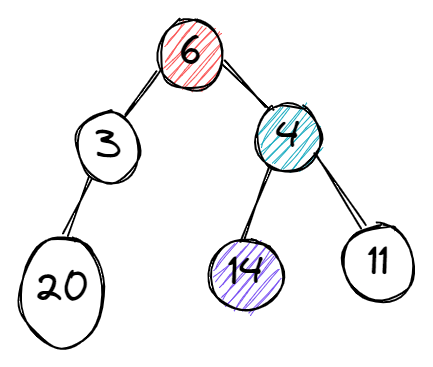
\includegraphics[width=0.3\linewidth]{Images/greedy.png}
    \caption{Thuật toán tham lam đi xác định điểm phù hợp gần nhất là điểm tối ưu}
    \label{fig:descGreedy}
\end{figure}

\subsubsubsection{Thuật toán sinh cột (Column Generation)}

\hspace{0.5cm}Sinh cột là một kỹ thuật phân rã mạnh mẽ, thường được sử dụng để giải các bài toán quy hoạch tuyến tính và tối ưu hóa tổ hợp quy mô lớn. Phương pháp này lặp đi lặp lại tinh chỉnh giải pháp bằng cách tạo ra các biến (cột) cải thiện hàm mục tiêu \cite{lubbecke2003columngeneration}.

\begin{itemize}
    \item \textbf{Cách hoạt động}: Phương pháp bắt đầu với một bài toán bị hạn chế chỉ bao gồm một tập hợp con của các biến. Một bài toán phụ định giá xác định các biến mới có tiềm năng nâng cao giải pháp. Các biến này được thêm vào lặp đi lặp lại cho đến khi không thể cải thiện thêm.
    \item \textbf{Ưu điểm}: Bằng cách tập trung vào một tập hợp con các biến tại mỗi lần lặp, sinh cột giúp giải quyết các bài toán với tập biến có kích thước lớn theo cấp số mũ.
    \item \textbf{Hạn chế}: Hiệu quả của sinh cột phụ thuộc vào việc giải quyết bài toán phụ định giá, điều này có thể trở nên khó khăn về mặt tính toán.
\end{itemize}

\begin{figure}[!htp]
    \centering
    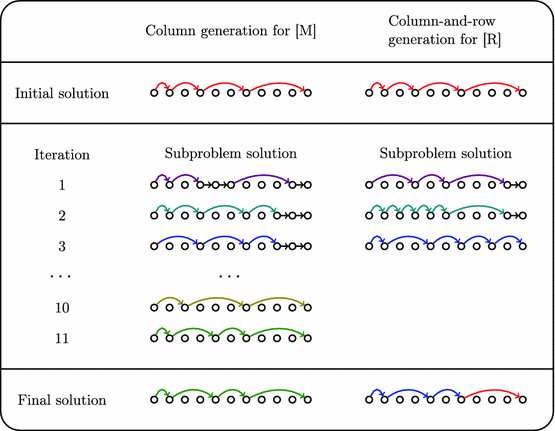
\includegraphics[width=0.35\linewidth]{Images/columngen.png}
    \caption{Quy trình sinh cột: Thêm biến lặp đi lặp lại}
    \label{fig:descColumnGen}
\end{figure}

\subsubsubsection{Thuật toán phân bổ tốt nhất (Best-Fit Algorithm)}
\hspace{0.5cm}Thuật toán phân bổ tốt nhất là một heuristic phổ biến trong việc giải quyết các bài toán đóng gói và phân bổ. Nó cố gắng tối thiểu hóa không gian lãng phí bằng cách đặt từng mục vào thùng hoặc ngăn phù hợp nhất \cite{cao2011bestfit}.

\begin{itemize}
    \item \textbf{Cách hoạt động}:
        \begin{itemize}
            \item Các mục được xử lý tuần tự.
            \item Mỗi mục được đặt vào thùng hoặc ngăn có không gian trống ít nhất mà vẫn đủ chứa mục.
            \item Nếu không tìm được thùng hoặc ngăn phù hợp, một thùng mới được mở.
        \end{itemize}
    \item \textbf{Ưu điểm}: Kỹ thuật này đơn giản và hiệu quả trong nhiều trường hợp thực tế.
    \item \textbf{Hạn chế}: Phương pháp có thể tạo ra các giải pháp kém tối ưu khi kích thước mục thay đổi hoặc các mục được xử lý không đồng nhất.
\end{itemize}





\section{Mô hình cho bài toán cắt tấm hai chiều}
\subsection{Mô tả bài toán}

\hspace{0.5cm} Cho một tập hợp gồm \( n \) miếng hình chữ nhật cần cắt với kích thước \( w_1 \times l_1, w_2 \times l_2, \dots, w_n \times l_n \), và nhu cầu tương ứng \( d_1, d_2, \dots, d_n \). Nhiệm vụ là cắt các miếng này từ \( m \) tấm vật liệu có kích thước \( W_1 \times L_1, W_2 \times L_2, \dots, W_m \times L_m \), với giả định rằng các tấm vật liệu đủ để đáp ứng nhu cầu cắt đặt ra. Tất cả các đường cắt phải theo các đường thẳng vuông góc, đảm bảo mỗi miếng được cắt thành hình chữ nhật nguyên vẹn.

Mục tiêu của bài toán là xây dựng một kế hoạch cắt tối ưu nhằm giảm thiểu lãng phí vật liệu, cụ thể là tối ưu hóa số lượng tấm vật liệu cần sử dụng để đáp ứng yêu cầu cắt.

Bài toán có thể được phân thành hai trường hợp chính:
\begin{itemize}
    \item \textbf{Kích thước tấm đồng nhất:} Tất cả các tấm vật liệu có kích thước giống nhau, giúp đơn giản hóa quy trình cắt nhưng vẫn đòi hỏi lập kế hoạch tối ưu.
    \item \textbf{Kích thước tấm không đồng nhất:} Các tấm vật liệu có kích thước khác nhau, làm tăng độ phức tạp vì cần xem xét đặc tính của từng loại tấm vật liệu.
\end{itemize}

Các ràng buộc chính bao gồm đảm bảo rằng tất cả các đường cắt đều vuông góc, không có sự chồng lấn giữa các miếng, và nhu cầu của mỗi loại miếng được đáp ứng đầy đủ.

\subsection{Mô hình đơn giản}
\subsubsection{Các biến và tham số}

\textbf{Tham số}

\begin{itemize}
    \item \( n \): Số lượng miếng cần cắt.
    \item \( m \): Số lượng tấm vật liệu sẵn có.
    \item \( w_p, l_p \): Chiều rộng và chiều dài của miếng \( p \) (\( p \in [1, n] \)).
    \item \( d_p \): Nhu cầu của miếng \( p \).
    \item \( W_s, L_s \): Chiều rộng và chiều dài của tấm vật liệu \( s \) (\( s \in [1, m] \)) (cho trường hợp nhiều kích thước tấm).
    \item \( I_{ps} = W_s - w_p + 1 \): Số vị trí khả thi theo trục ngang trên tấm \( s \) để đặt miếng \( p \).
    \item \( J_{ps} = L_s - l_p + 1 \): Số vị trí khả thi theo trục dọc trên tấm \( s \) để đặt miếng \( p \).
\end{itemize}

\textbf{Biến quyết định}

\( x_{spij} \): Biến nhị phân, chỉ ra rằng miếng \( p \) được đặt trên tấm \( s \) tại vị trí \((i, j)\), tức tọa độ góc dưới bên trái.

\( y_s , \quad \forall s \in \{1, 2, \dots, m\} \): \( y_s = 1 \) nếu tấm \( s \) được sử dụng (ít nhất một miếng được đặt lên đó), và \( y_s = 0 \) nếu tấm \( s \) không được sử dụng.

\subsubsection{Hàm mục tiêu}

Mục tiêu là giảm thiểu diện tích của các tấm vật liệu được sử dụng.

Diện tích lãng phí của tấm \( s \) là phần không sử dụng:  
\[
\text{Waste}_s = L_s \cdot W_s - \sum_{p=1}^n \sum_{i=1}^{I_{ps}} \sum_{j=1}^{J_{ps}} x_{psij} \cdot w_p \cdot l_p
\]  
Hàm mục tiêu:  
\[
\text{Minimize} \quad \sum_{s=1}^m y_s \cdot \left(L_s \cdot W_s - \sum_{p=1}^n \sum_{i=1}^{I_{ps}} \sum_{j=1}^{J_{ps}} x_{psij} \cdot w_p \cdot l_p \right)
\]  
Hoặc tương đương:  
\[
\text{Minimize} \quad \sum_{s=1}^m y_s \cdot L_s \cdot W_s - \sum_{s=1}^m \sum_{p=1}^n \sum_{i=1}^{I_{ps}} \sum_{j=1}^{J_{ps}} x_{psij} \cdot w_p \cdot l_p
\]

\subsubsection{Các ràng buộc}

\begin{enumerate}

\item \textbf{Ràng buộc không chồng lấn}

Tổng các biến \( x_{psij} \) cho tất cả các miếng \( p \) tại bất kỳ ô lưới nào \((i, j)\) trên tấm \( s \) không được vượt quá 1, nghĩa là một ô lưới không thể bị chồng lấn bởi nhiều miếng.  
\[
\sum_{p=1}^{n} \sum_{i=\max(0, u - l_p + 1)}^{\min(L_s - l_p, u)} \sum_{l=\max(0, v - w_p + 1)}^{\min(W_s - w_p, v)} x_{psij} \leq 1, \quad \forall s \in [1,2,...,m], \forall u, v
\]

\item \textbf{Ràng buộc trong giới hạn}

Đảm bảo rằng miếng \( p \) không vượt ra ngoài ranh giới của tấm \( s \). Nếu vị trí đặt vượt quá biên của tấm, biến quyết định \( x_{psij} \) phải bằng 0.  
\[
x_{psij} \leq \left( 1 - \mathbb{I}\left( i + l_p > L_s \right) \right), \quad \forall s, p, i, j
\]  
\[
x_{psij} \leq \left( 1 - \mathbb{I}\left( j + w_p > W_s \right) \right), \quad \forall s, p, i, j
\]

\item \textbf{Đáp ứng nhu cầu}

Đảm bảo tất cả các nhu cầu đều được đáp ứng:  
\[
\sum_{s=1}^{m} \sum_{i=1}^{I_{ps}} \sum_{j=1}^{J_{ps}} x_{psij} \geq d_p, \quad \forall p \in \{1, 2, \dots, n\} 
\]

\textbf{Ràng buộc nhị phân}
Tất cả các biến quyết định phải tuân thủ giá trị logic:  
\[
x_{psij}\in \{0, 1\}, \quad \forall s, p, i ,j
\]  
\[
y_s \in \{0, 1\}
\]

\end{enumerate}

\subsubsection{Đánh giá mô hình}
\hspace{0.5cm} Mô hình này rõ ràng và có cấu trúc tốt về mặt lý thuyết. Tuy nhiên, việc triển khai thực tế sẽ yêu cầu một lượng lớn biến quyết định (biến nhị phân). Cụ thể, mỗi biến xác định xem miếng \( p \) có được đặt trên tấm \( s \) tại vị trí \( i, j \) hay không. Do đó, tổng số biến quyết định cần thiết là \( n \times m \times \sum_{i=1}^m L_i \times W_i \). Điều này làm tăng độ phức tạp tính toán của mô hình, đặc biệt trong các trường hợp có số lượng miếng hoặc vị trí lớn.

\subsection{Mô hình thu gọn}  
\hspace{0.5cm}Mô hình này được lấy cảm hứng từ công trình của Fabio Furini trong bài báo đăng trên *Computers \& Operations Research* (tháng 8 năm 2013) \cite{furini2013cuttingstock}. Mục tiêu của mô hình là sử dụng Lập trình hỗn hợp số nguyên (MIP) để giải các bài toán tối ưu hóa.  

\subsubsection{Biến và tham số}  
\begin{itemize}  
    \item \textbf{Tham số:}  
    \begin{itemize}  
        \item $n$: Tổng số loại sản phẩm cần cắt.  
        \item $d_j$: Nhu cầu của loại sản phẩm $j$, với $j = 1, \dots, n$.  
        \item $w_i$: Chiều rộng của sản phẩm $i$, với $i = 1, \dots, n$, được sắp xếp theo thứ tự giảm dần ($w_1 \geq w_2 \geq \dots \geq w_n$).  
        \item $l_i$: Chiều dài của sản phẩm $i$, với $i = 1, \dots, n$.  
        \item $A_h$: Diện tích của một tấm nguyên liệu loại $h$, với $h = 1, \dots, p$.  
        \item $L_h, W_h$: Chiều dài và chiều rộng của một tấm nguyên liệu loại $h$.  
    \end{itemize}  
    \item \textbf{Biến:}  
    \begin{itemize}  
        \item $y_i^h$: Biến nhị phân; bằng 1 nếu sản phẩm $i$ khởi tạo mức $i$ trong tấm nguyên liệu loại $h$.  
        \item $x_{ij}^h$: Biến nguyên; số lượng sản phẩm loại $j$ được sắp xếp vào mức $i$ trong tấm nguyên liệu loại $h$.  
        \item $q_k^h$: Biến nhị phân; bằng 1 nếu mức $k$ khởi tạo tấm nguyên liệu $k$ loại $h$.  
        \item $z_{ki}^h$: Biến nhị phân; bằng 1 nếu mức $i$ được gán cho tấm nguyên liệu $k$ loại $h$.  
    \end{itemize}  
\end{itemize}  

\subsubsection{Hàm mục tiêu}  
Tối thiểu hóa tổng diện tích của các tấm nguyên liệu được sử dụng:  
\[
\min \sum_{h=1}^{p} A_h \sum_{k=1}^{n} q_k^h
\]  

\subsubsection{Các ràng buộc}  
\begin{enumerate}  
    \item \textbf{Đáp ứng nhu cầu:} Đảm bảo rằng nhu cầu của mỗi loại sản phẩm được đáp ứng:  
    \[
    \sum_{h=1}^{p} \left( \sum_{i=1}^{j} x_{ij}^h + \sum_{i=j}^{n} y_i^h \right) \geq d_j, \quad j = 1, \dots, n.
    \]  

    \item \textbf{Ràng buộc chiều rộng:} Đảm bảo chiều rộng của mức không vượt quá chiều rộng của tấm nguyên liệu:  
    \[
    \sum_{j=i}^{n} l_j x_{ij}^h \leq (L_h - l_i) y_i^h, \quad i = 1, \dots, n-1; \, h = 1, \dots, p.
    \]  

    \item \textbf{Phân bổ mức:} Mỗi mức khởi tạo hoặc là một tấm nguyên liệu mới hoặc là một phần của tấm nguyên liệu hiện có:  
    \[
    \sum_{k=1}^{i-1} z_{ki}^h + q_i^h = y_i^h, \quad i = 1, \dots, n; \, h = 1, \dots, p.
    \]  

    \item \textbf{Ràng buộc chiều cao:} Đảm bảo chiều cao của tấm nguyên liệu không vượt quá giới hạn:  
    \[
    \sum_{i=k+1}^{n} w_i z_{ki}^h \leq (W_h - w_k) q_k^h, \quad k = 1, \dots, n-1; \, h = 1, \dots, p.
    \]  

    \item \textbf{Miền giá trị của biến:}  
    \[
    y_i^h, q_k^h, z_{ki}^h \in \{0, 1\}, \quad x_{ij}^h \geq 0.
    \]  
\end{enumerate}  

\subsection{Mô hình tối ưu hóa mẫu cắt}  

\subsubsection{Biến và tham số}  
\begin{itemize}  
    \item \textbf{Tham số:}  
    \begin{itemize}  
        \item $N$: Số loại sản phẩm cần cắt.  
        \item $K$: Số loại chiều rộng của cuộn nguyên liệu.  
        \item $w_i$: Chiều rộng của sản phẩm $i$, với $i = 1, \dots, N$.  
        \item $l_i$: Chiều dài của sản phẩm $i$, với $i = 1, \dots, N$.  
        \item $d_i$: Nhu cầu của sản phẩm $i$, với $i = 1, \dots, N$.  
        \item $W_k$: Chiều rộng tiêu chuẩn của cuộn loại $k$, với $k = 1, \dots, K$.  
        \item $J_k$: Số mẫu cắt cho cuộn có chiều rộng $W_k$.  
    \end{itemize}  

    \item \textbf{Biến:}  
    \begin{itemize}  
        \item $V_{kji}$: Số lượng sản phẩm có chiều rộng $w_i$ được cắt bằng mẫu cắt thứ $j$ trên cuộn loại $k$.  
        \item $L_{kj}$: Chiều dài được sản xuất bằng mẫu cắt thứ $j$ trên cuộn loại $k$.  
    \end{itemize}  
\end{itemize}  

\subsubsection{Hàm mục tiêu}  
Tối thiểu hóa tổng diện tích sử dụng từ tất cả các cuộn, tương đương với việc giảm thiểu lượng phế liệu:  
\[
\min \sum_{k=1}^{K} \sum_{j=1}^{J_k} W_k L_{kj}
\]  

\subsubsection{Các ràng buộc}  
\begin{enumerate}  
    \item \textbf{Đáp ứng nhu cầu:} Đảm bảo nhu cầu của mỗi loại sản phẩm được đáp ứng:  
    \[
    \sum_{k=1}^{K} \sum_{j=1}^{J_k} V_{kji} \geq d_i, \quad i = 1, \dots, N.
    \]  

    \item \textbf{Tính khả thi của mẫu cắt:} Tổng chiều rộng của các sản phẩm trong một mẫu không được vượt quá chiều rộng cuộn:  
    \[
    \sum_{i=1}^{N} V_{kji} w_i \leq W_k, \quad k = 1, \dots, K; \, j = 1, \dots, J_k.
    \]  

    \item \textbf{Mẫu không bị chi phối:} Các mẫu được chọn dựa trên chiều rộng cuộn khả thi gần nhất:  
    \[
    W_{k-1} < \sum_{i=1}^{N} V_{kji} w_i \leq W_k, \quad k = 1, \dots, K; \, j = 1, \dots, J_k.
    \]  

    \item \textbf{Không âm:} Tất cả các biến phải không âm:  
    \[
    L_{kj} \geq 0, \quad k = 1, \dots, K; \, j = 1, \dots, J_k.
    \]  
\end{enumerate}  
\section{Những thuật toán Heuristic giải quyết 2DCSP}
\subsection{Tạo Cột (Generate Column)}

\hspace{0.5cm}Bài toán cắt hai chiều (2DCSP) liên quan đến việc cắt nguyên liệu thành các mảnh nhỏ hơn để đáp ứng nhu cầu sản phẩm được chỉ định, đồng thời giảm thiểu lãng phí. Đây là một bài toán phức tạp về tổ hợp, đòi hỏi các chiến lược động để giải quyết hiệu quả các trường hợp quy mô lớn. Thuật toán được trình bày tạo mẫu cắt động và ưu tiên bố trí dựa trên kích thước sản phẩm và khả năng nguyên liệu sẵn có.

Thuật toán bao gồm các thành phần chính sau:

\textbf{Tạo mẫu động}

Thuật toán tạo các mẫu cắt động dựa trên kích thước và số lượng sản phẩm còn lại. Các sản phẩm được sắp xếp theo thứ tự giảm dần diện tích (\( \text{Width} \times \text{Height} \)) để ưu tiên các sản phẩm lớn hơn. Quá trình tạo mẫu điền lần lượt các mẫu bằng cách xem xét các vị trí khả thi cho từng sản phẩm.

Gọi \( P = \{p_1, p_2, \dots, p_n\} \) là tập hợp các sản phẩm, trong đó mỗi sản phẩm \( p_i \) có:
\[
\text{Kích thước}(p_i) = (w_i, l_i), \quad \text{Số lượng}(p_i) = d_i
\]

Các mẫu cắt được biểu diễn như sau:
\[
\text{Mẫu} = \{x_1, x_2, \dots, x_n\}, \quad x_i \text{ là số mảnh của } p_i \text{ trong mẫu}.
\]

Với mỗi sản phẩm \( p_i \), số lượng tối đa các mảnh có thể đặt trong nguyên liệu kích thước \( (W, H) \) là:
\[
\text{Số lượng tối đa}(p_i) = \min\left(q_i, \left\lfloor \frac{W}{w_i} \right\rfloor \times \left\lfloor \frac{H}{h_i} \right\rfloor\right).
\]

Để bố trí sản phẩm vào nguyên liệu, thuật toán xác định các vị trí khả thi bằng cách duyệt qua tất cả các tọa độ \( (x, y) \) trong nguyên liệu. Một vị trí là hợp lệ nếu sản phẩm không chồng lấn với các mảnh đã được đặt trước đó và nằm trong giới hạn kích thước của nguyên liệu.

Gọi \( S \) là nguyên liệu kích thước \( (W, H) \), và gọi \( p_i \) là sản phẩm kích thước \( (w_i, h_i) \). Một vị trí \( (x, y) \) là hợp lệ nếu:
\[
x + w_i \leq W, \quad y + h_i \leq H, \quad \text{và không chồng lấn với các mảnh đã đặt trước đó}.
\]

\textbf{Ưu tiên nguyên liệu}

Nguyên liệu được sắp xếp theo thứ tự giảm dần diện tích để ưu tiên các nguyên liệu lớn hơn cho việc bố trí:
\[
\text{Ưu tiên nguyên liệu} = \text{Diện tích}(S) = W \times H.
\]

\textbf{Quy trình thuật toán}

Quy trình được tóm tắt như sau:
\begin{enumerate}[1) ]
    \item Sắp xếp các sản phẩm theo diện tích giảm dần.

    \item Sắp xếp các nguyên liệu theo diện tích giảm dần.

    \item Tạo các mẫu cắt động cho nguyên liệu lớn nhất.

    \item Duyệt qua các mẫu để bố trí sản phẩm vào nguyên liệu:

    \begin{enumerate}
        \item Kiểm tra nếu tồn tại vị trí hợp lệ cho từng sản phẩm trong mẫu.
        \item Nếu tìm thấy vị trí, đặt sản phẩm và cập nhật việc sử dụng nguyên liệu.
    \end{enumerate}
   
    \item Nếu không tìm thấy vị trí hợp lệ, chuyển sang nguyên liệu tiếp theo.

    \item Lặp lại cho đến khi tất cả nhu cầu sản phẩm được đáp ứng hoặc nguyên liệu đã hết.
\end{enumerate}

\begin{figure}[!htp]
    \centering
    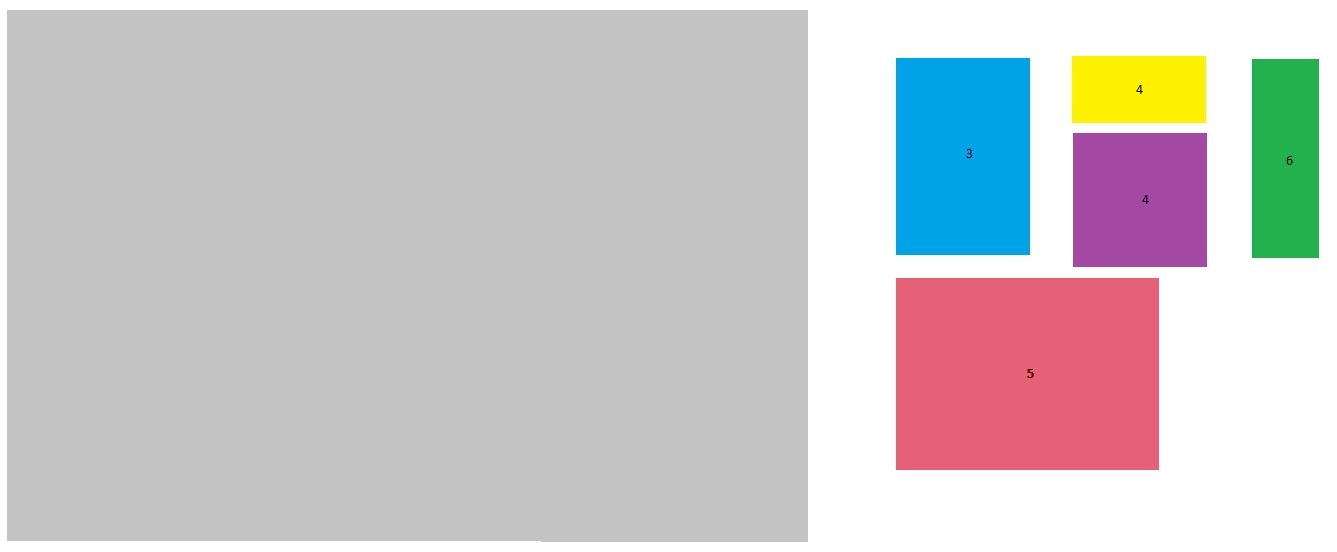
\includegraphics[width=0.5\linewidth]{Images/gencolumn.png}
    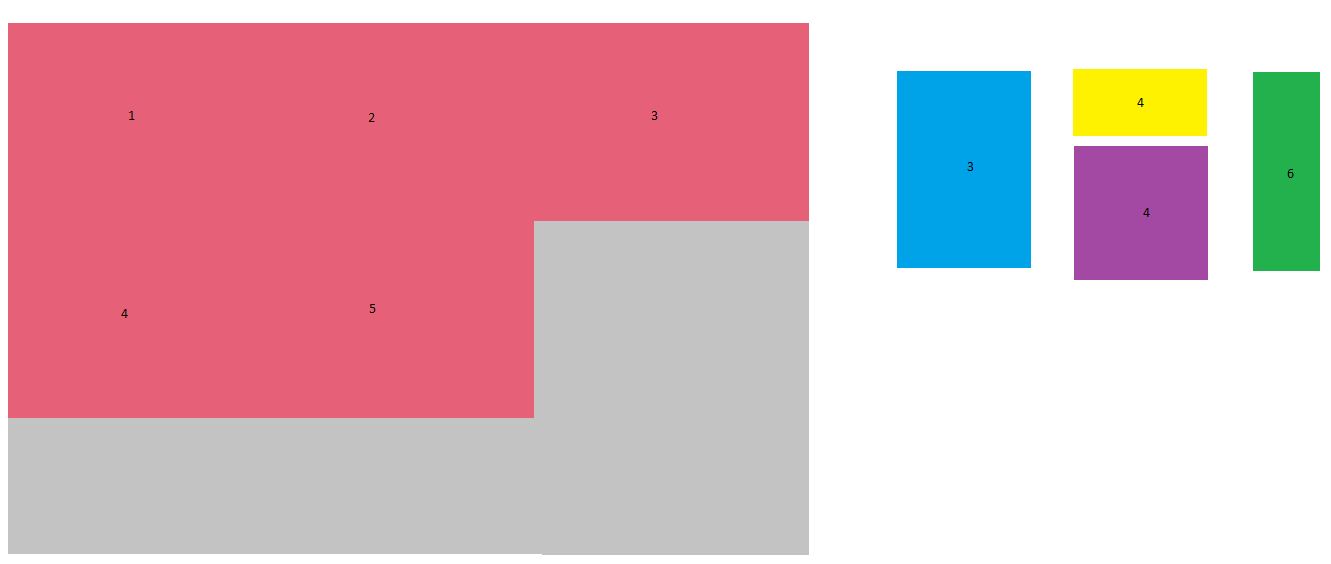
\includegraphics[width=0.5\linewidth]{Images/gencolumn_res.png}
    \caption{Bố trí một nguyên liệu sau khi áp dụng thuật toán Generate Column.}
    \label{fig:stock-layout}
\end{figure}

\subsection{Phân bổ Best-Fit với Lựa chọn Heuristic}

\hspace{0.5cm}\textbf{Thuật toán Best-Fit} là một giải pháp tối ưu cho việc sắp xếp sản phẩm lên các vật liệu tồn kho, được thiết kế tỉ mỉ nhằm giảm thiểu lãng phí và tối đa hóa hiệu suất sử dụng. Bằng cách kết hợp các quyết định lặp lại với cơ chế chấm điểm tiên tiến, thuật toán xác định cách bố trí hiệu quả nhất cho từng sản phẩm. Phần này sẽ trình bày nguyên tắc cơ bản, quy trình hoạt động, và các ưu điểm của thuật toán trong thực tế.

\vspace{0.3cm}
\noindent\textbf{Nguyên tắc cơ bản}

Thuật toán dựa trên \textit{chiến lược đặt sản phẩm theo đường bao (skyline-based placement strategy)} để xác định vị trí tối ưu cho từng sản phẩm, với các tiêu chí sau:
\begin{enumerate}
    \item \textbf{Hiệu suất sử dụng diện tích:} Ưu tiên sắp xếp các sản phẩm sao cho giảm thiểu không gian chưa sử dụng.
    \item \textbf{Căn chỉnh chiều cao:} Đảm bảo các sản phẩm được sắp xếp theo chiều dọc để tạo sự gọn gàng.
    \item \textbf{Ưu tiên căn chỉnh theo cạnh:} Khuyến khích sắp xếp sản phẩm dọc theo các cạnh của vật liệu để giảm sự phân mảnh.
    \item \textbf{Theo dõi hiệu suất sử dụng:} Giám sát tỷ lệ diện tích đã sử dụng để tối ưu hóa hiệu suất vật liệu.
\end{enumerate}

\vspace{0.3cm}
\noindent\textbf{Quy trình hoạt động}

Thuật toán Best-Fit hoạt động theo các bước sau:

\begin{enumerate}[1) ]
    \item \textbf{Khởi tạo:} Thiết lập các cấu trúc dữ liệu để theo dõi:
    \begin{itemize}
        \item \textbf{Hiệu suất sử dụng từng vật liệu:} Tỷ lệ phần trăm diện tích đã sử dụng.
        \item \textbf{Các vị trí đã chiếm:} Các tọa độ trong vật liệu đã được sử dụng.
        \item \textbf{Các tham số:} Như ngưỡng lãng phí và tỷ lệ chiều cao tối đa.
    \end{itemize}
    \item \textbf{Tính toán đường bao (Skyline):} Xây dựng hồ sơ đường bao cho mỗi vật liệu:
    \[
    \text{Skyline}[i] = \max(\text{tọa độ y được chiếm tại } x = i)
    \]
    \begin{figure}[!htp]
        \centering
        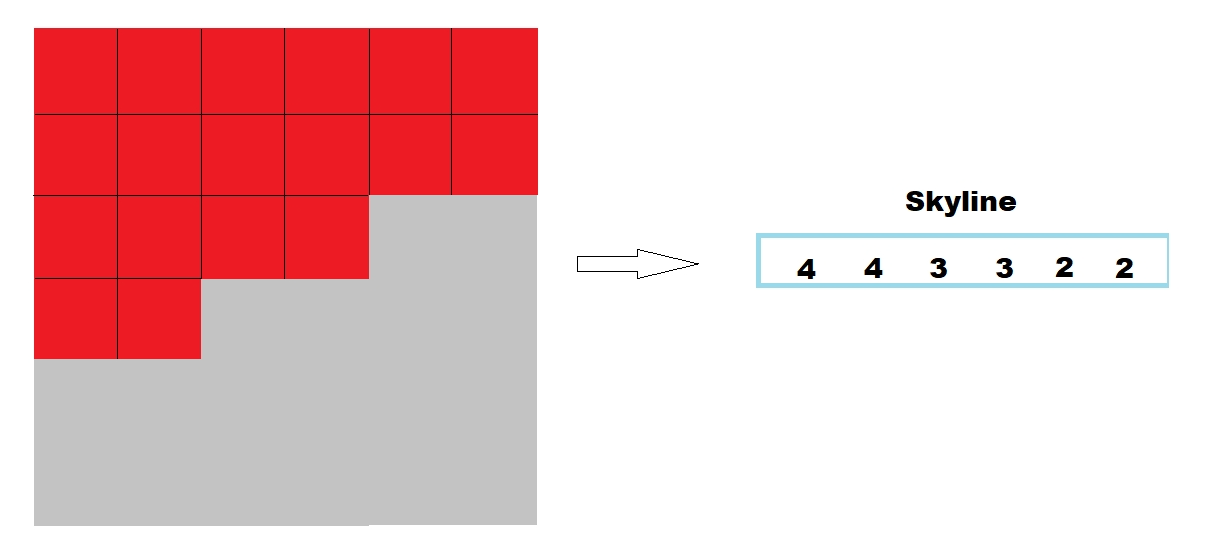
\includegraphics[width=0.4\linewidth]{Images/skyline.png}
        \caption{Hồ sơ đường bao của một vật liệu đã sử dụng}
        \label{fig:enter-label}
    \end{figure}
    Hồ sơ này giúp xác định không gian theo chiều dọc còn trống tại mỗi vị trí ngang.
    \item \textbf{Chiến lược đặt sản phẩm:} 
    \begin{enumerate}[a)]
        \item Sắp xếp các sản phẩm theo thứ tự giảm dần của diện tích (\( \text{Width} \times \text{Height} \)).
        \item Với mỗi sản phẩm, đánh giá các vị trí khả thi dựa trên hồ sơ đường bao.
        \item Gán điểm số cho từng vị trí dựa trên:
        \begin{itemize}
            \item \textit{Lãng phí diện tích:} Không gian không sử dụng xung quanh sản phẩm.
            \item \textit{Phạt chiều cao:} Sự không đều về chiều cao so với đường bao hiện tại.
            \item \textit{Thưởng căn chỉnh cạnh:} Khuyến khích căn chỉnh sản phẩm theo các cạnh của vật liệu.
            \item \textit{Thưởng hiệu suất sử dụng:} Điểm cao hơn cho việc tối đa hóa không gian được lấp đầy.
        \end{itemize}
        \item Chọn vị trí có điểm số lãng phí thấp nhất.
    \end{enumerate}
    \item \textbf{Cập nhật trạng thái:} Sau khi đặt sản phẩm:
    \begin{itemize}
        \item Cập nhật các vị trí đã chiếm và hồ sơ đường bao của vật liệu.
        \item Điều chỉnh thống kê hiệu suất sử dụng của vật liệu.
    \end{itemize}
    \item \textbf{Kết thúc:} Lặp lại cho đến khi tất cả sản phẩm được đặt hoặc không còn vị trí khả thi.
\end{enumerate}

\vspace{0.3cm}
\noindent\textbf{Tính toán lãng phí}

Thuật toán tính \textbf{điểm số lãng phí} để đánh giá các vị trí khả thi:
\[
\text{Điểm số lãng phí} = 
\]
\[
(1 - \text{Hiệu suất sử dụng diện tích}) + \text{Phạt chiều cao} - \text{Thưởng căn chỉnh cạnh} - \text{Thưởng hiệu suất sử dụng}
\]
Điểm số này cân bằng nhiều yếu tố để xác định vị trí sắp xếp hiệu quả nhất.

\vspace{0.3cm}
\noindent\textbf{Ưu điểm của thuật toán Best-Fit}
\begin{itemize}
    \item \textbf{Chiến lược thích ứng:} Linh hoạt điều chỉnh vị trí đặt dựa trên hồ sơ vật liệu.
    \item \textbf{Hiệu quả vật liệu:} Giảm thiểu lãng phí và đạt tỷ lệ sử dụng cao.
    \item \textbf{Khả năng mở rộng:} Xử lý hiệu quả số lượng lớn sản phẩm và kích thước vật liệu đa dạng.
\end{itemize}

Bằng cách tích hợp liền mạch các phương pháp đường bao với hệ thống chấm điểm tiên tiến, thuật toán Best-Fit cung cấp một giải pháp mạnh mẽ và mở rộng để giải quyết bài toán sắp xếp sản phẩm, đảm bảo tối ưu hóa sử dụng vật liệu và giảm thiểu lãng phí.
\section{Thực nghiệm và phân tích kết quả}
\subsection{Các chỉ số chính để đánh giá hiệu quả của bài toán 2DCSP}

\hspace{0.5cm}Để đánh giá hiệu quả của các thuật toán giải 2DCSP, chúng ta xem xét các chỉ số chính sau:

\begin{itemize}
    \item \textbf{Mức độ lãng phí vật liệu:} Đánh giá tỷ lệ phần trăm diện tích vật liệu đầu vào được sử dụng hiệu quả. Chỉ số này được tính bằng công thức:
    \[
    \text{Mức độ lãng phí vật liệu} = \frac{\text{Tổng diện tích các mảnh cắt}}{\text{Tổng diện tích vật liệu đã sử dụng}} \times 100\%.
    \]
    Giá trị càng thấp thể hiện khả năng sử dụng vật liệu càng hiệu quả.
    
    Giá trị vật liệu càng thấp chứng tỏ mẫu cắt được tối ưu hơn.

    \item \textbf{Thời gian tính toán:} Thời gian mà thuật toán cần để tìm ra lời giải, đặc biệt quan trọng khi đánh giá khả năng mở rộng đối với các tập dữ liệu lớn.

    \item \textbf{Đáp ứng nhu cầu sản phẩm:} Đánh giá mức độ đáp ứng nhu cầu sản xuất bằng cách kiểm tra số lượng sản phẩm đã thực hiện cắt.

    \item \textbf{Giảm thiểu số lượng tấm vật liệu:} So sánh tổng số tấm vật liệu được sử dụng với số lượng tối thiểu lý thuyết cần thiết.
\end{itemize}

\subsubsection{Tóm tắt các chỉ số chính}

Bảng dưới đây tóm tắt các chỉ số chính để đánh giá hiệu quả của các thuật toán:

\begin{table}[H]
    \centering
    \renewcommand{\arraystretch}{1.5}
    \begin{tabular}{|l|p{1.5cm}|p{6cm}|p{1.3cm}|}
     \hline
        \textbf{Chỉ số}               & \textbf{Đơn vị}                 & \textbf{Mô tả}                                                                                 & \textbf{Mức độ quan trọng}  \\ \hline
        Mức độ lãng phí vật liệu    & \%                            & tỷ lệ phần trăm diện tích vật liệu đầu vào được sử dụng
hiệu quả.                                          & Cao \\ \hline
        Thời gian tính toán           & giây                          & Thời gian cần để tính toán lời giải.                                                            & Vừa                   \\ \hline
        Đáp ứng nhu cầu               & sản phẩm                            & Số lượng nhu cầu sản phẩm được đáp ứng.                                                            & Vừa  \\ \hline
        Số lượng tấm vật liệu         & \text{tấm}                    & Tổng số tấm vật liệu sử dụng so với số lượng tối thiểu lý thuyết.                               & Cao                   \\ \hline
    \end{tabular}
    \caption{Các chỉ số chính để đánh giá hiệu quả của bài toán 2DCSP}
    \label{tab:key_metrics}
\end{table}

\subsection{Đánh giá kết quả thực nghiệm}
\subsubsection{Môi trường thực nghiệm}

Các thử nghiệm được thực hiện trên một hệ thống có cấu hình như sau:

\begin{itemize}
    \item \textbf{Hệ điều hành (OS):} Windows 10 Pro, phiên bản Build 22H2 (19045).
    \item \textbf{Độ phân giải màn hình:} 1920x1080 @60Hz.
    \item \textbf{Bộ xử lý (CPU):} Intel(R) Core(TM) i7-8550U CPU @ 1.80GHz.
    \item \textbf{Đồ họa (GPU):} Intel(R) UHD Graphics 620.
    \item \textbf{Bộ nhớ (RAM):} 8493 MB / 16278 MB (52\% đang sử dụng).
    \item \textbf{Dung lượng đĩa (Disk):} Ổ đĩa C:\ có tổng dung lượng 104.84 GB (còn trống 11.07 GB).
\end{itemize}

Chúng tôi sử dụng ngôn ngữ lập trình Python để mô phỏng và kiểm thử hai thuật toán nói trên trên cùng tập dữ liệu. Tập dữ liệu được sử dụng có thể truy cập tại liên kết sau: \href{https://raw.githubusercontent.com/nhan2892005/ReinforcementLearning/refs/heads/main/CSP/results.csv}{Dữ liệu kiếm thử}.

Biểu đồ dưới đây minh họa phân bố dữ liệu trong quá trình kiểm thử:

\begin{figure}[H]
    \centering
    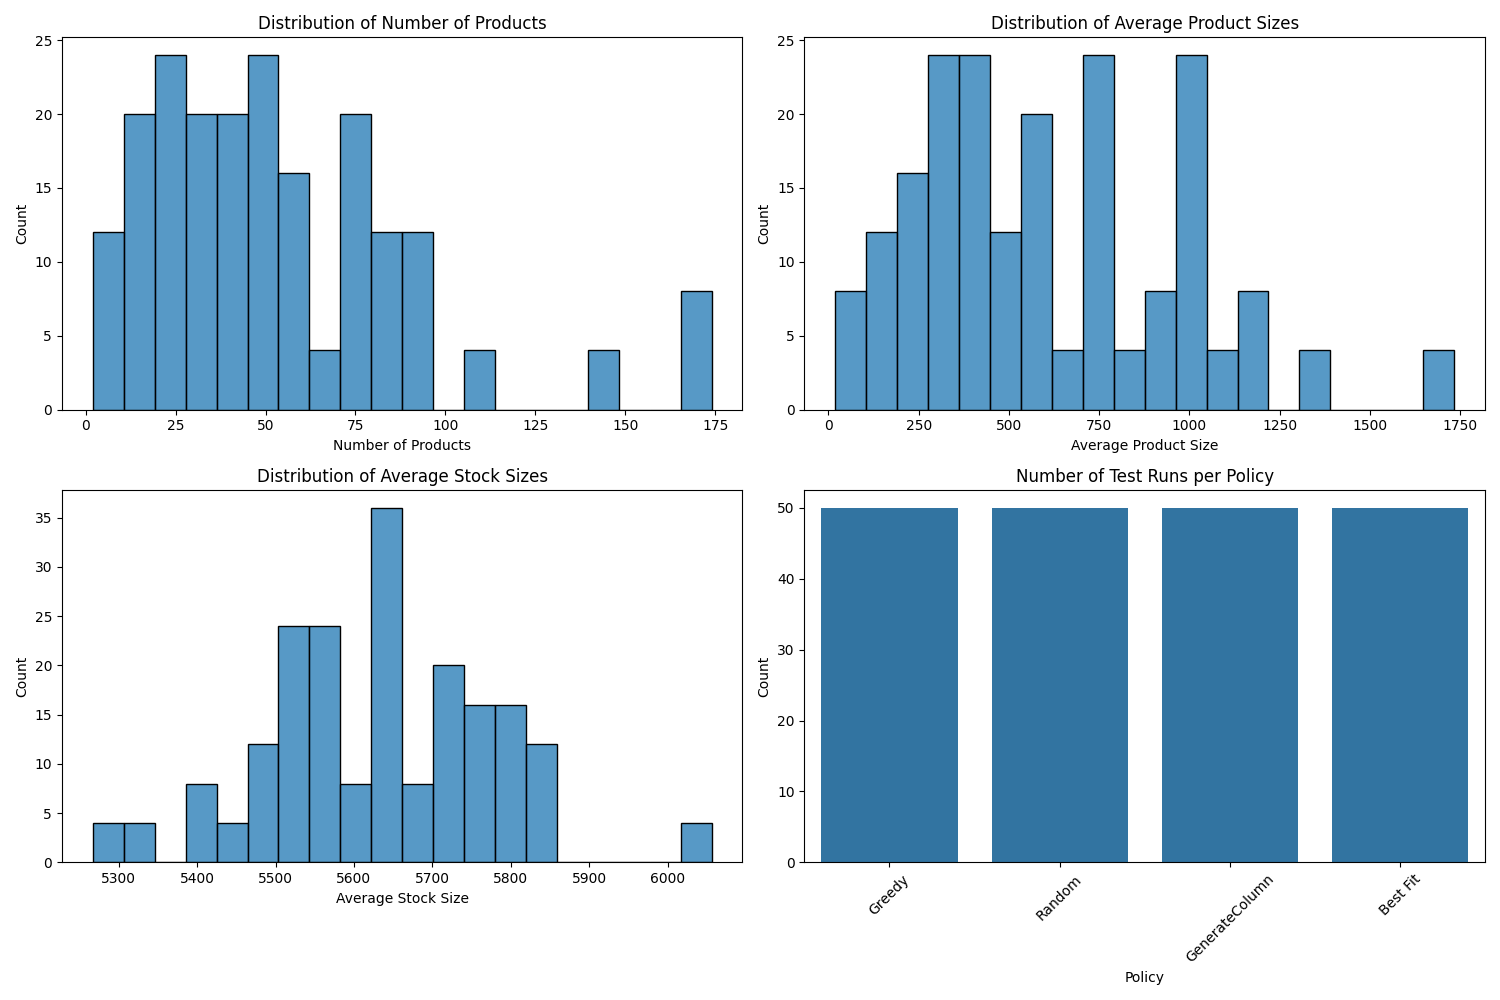
\includegraphics[width=0.8\textwidth]{Images/test_case_distributions.png}
    \caption{Phân bố số lượng sản phẩm, kích thước sản phẩm trung bình, kích thước kho trung bình, và số lần chạy thử nghiệm cho mỗi chính sách.}
    \label{fig:test_distributions}
\end{figure}

\textbf{Mô tả biểu đồ:}
\begin{itemize}
    \item \textbf{Phân bố số lượng sản phẩm:} Biểu đồ trên bên trái cho thấy số lượng sản phẩm được phân bố từ khoảng 0 đến 175 sản phẩm, với phần lớn rơi vào khoảng 25-75 sản phẩm.
    \item \textbf{Phân bố kích thước sản phẩm trung bình:} Biểu đồ trên bên phải minh họa các kích thước trung bình của sản phẩm, tập trung nhiều trong khoảng 250-1000 đơn vị.
    \item \textbf{Phân bố kích thước kho trung bình:} Biểu đồ dưới bên trái cho thấy kích thước kho trung bình dao động từ 5300 đến 6000 đơn vị, với phần lớn các trường hợp tập trung gần 5600 đơn vị.
    \item \textbf{Số lần chạy thử nghiệm:} Biểu đồ dưới bên phải thể hiện số lần thử nghiệm thực hiện cho từng chính sách. Tất cả các chính sách (Greedy, Random, GenerateColumn, và Best Fit) đều có số lần chạy thử nghiệm bằng nhau là 50 lần, và mỗi lần đều chạy trên cùng 1 bộ dữ liệu kiểm thử.
\end{itemize}

\subsubsection{Phân tích kết quả thí nghiệm}

Kết quả thí nghiệm được thể hiện qua bốn biểu đồ, bao gồm: \textit{Waste Percentage by Policy}, \textit{Number of Used Stocks by Policy}, \textit{Execution Time by Policy}, và \textit{Waste vs Number of Products}. Dưới đây là các phân tích chi tiết:


\begin{table}[!htp]
    \centering
    \begin{tabular}{|c|c|c|c|} \hline 
       \textbf{  Policy}&  \textbf{Avg Stock Use}d&  \textbf{Trim Loss} (\%)& \textbf{ Avg Runtime (s)}
\\ \hline 
         Best Fit&  5.4&  2.36&  2.106
\\ \hline 
         Generate Column&  5.08&  1.92&  10.560
\\ \hline 
         Greedy&  9.74&  3.08&  7.824
\\ \hline 
         Random&  41.14&  35.31&  0.009\\ \hline
    \end{tabular}
    \caption{Bảng số liệu giá trị trung bình các chỉ số của các thuật toán}
    \label{tab:result}
\end{table}

\begin{itemize}
    \item \textbf{Phần trăm lãng phí theo chính sách (Waste Percentage by Policy):} 
    \begin{itemize}
        \item Chính sách \textit{Greedy}, \textit{GenerateColumn}, và \textit{Best Fit} đều có phần trăm lãng phí thấp, với đa số giá trị tập trung gần mức 0-10\%. Điều này cho thấy ba chính sách này hiệu quả hơn trong việc giảm lãng phí.
        \item Ngược lại, chính sách \textit{Random} có sự biến thiên lớn và lãng phí cao hơn đáng kể, với mức trung bình dao động quanh 40\%. Đây là lựa chọn kém hiệu quả nhất.
    \end{itemize}

    \begin{figure}[!htp]
        \centering
        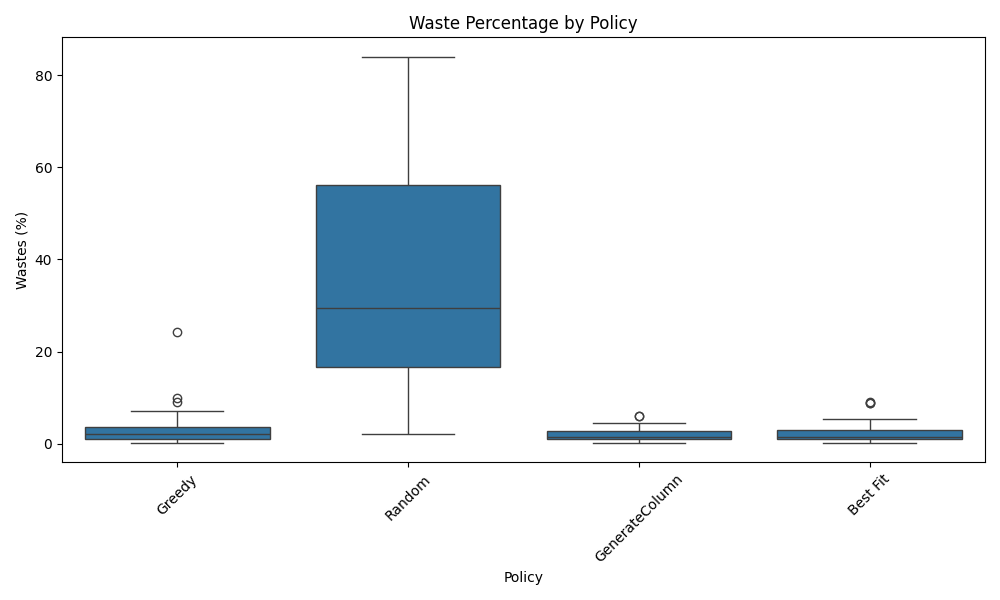
\includegraphics[width=0.5\linewidth]{Images/waste_comparison.png}
        \caption{Biểu đồ hộp thể hiện mức độ lãng phí trung bình của các chính sách}
        \label{fig:trimloss}
    \end{figure}
    
    \item \textbf{Số lượng vật liệu sử dụng theo chính sách (Number of Used Stocks by Policy):}
    \begin{itemize}
        \item Chính sách \textit{Greedy}, \textit{GenerateColumn}, và \textit{Best Fit} tiếp tục thể hiện sự ổn định, với số lượng kho sử dụng thấp và ít biến thiên.
        \item Chính sách \textit{Random} có số lượng vật liệu sử dụng lớn nhất và phân bố rộng, cho thấy sự có thể gây nhiều lãng phí trong việc tận dụng không gian lưu trữ.
    \end{itemize}
    \begin{figure}[!htp]
        \centering
        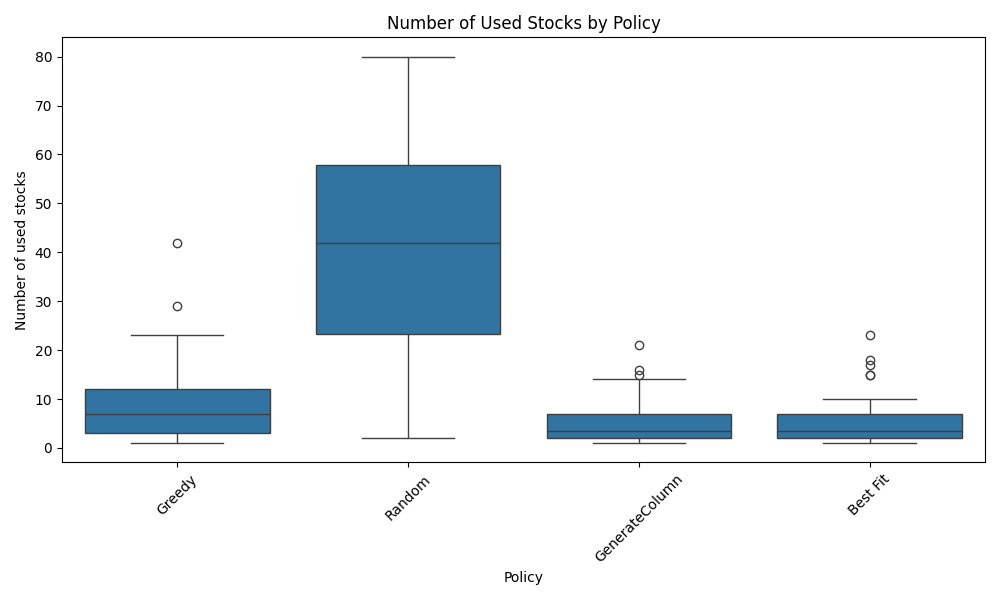
\includegraphics[width=0.5\linewidth]{Images/stocks_comparison.png}
        \caption{Biểu đồ hộp thể hiện số lượng vật liệu trung bình các chính sách sử dụng}
        \label{fig:stocks}
    \end{figure}
    
    \item \textbf{Thời gian thực thi theo chính sách (Execution Time by Policy):}
    \begin{itemize}
        \item Chính sách \textit{Greedy} và \textit{Best Fit} có thời gian thực thi thấp nhất, hầu hết dưới 5 giây. Điều này cho thấy chúng vừa hiệu quả về mặt chi phí lưu trữ, vừa nhanh về thời gian xử lý.
        \item Chính sách \textit{Generate Column} có thời gian thực thi cao hơn, với một số trường hợp cao gấp 5 lần trở lên so với các thuật toán khác. Mặc dù hiệu quả giảm lãng phí tốt, thời gian thực thi là một nhược điểm cần lưu ý.
    \end{itemize}
    \begin{figure}[!htp]
        \centering
        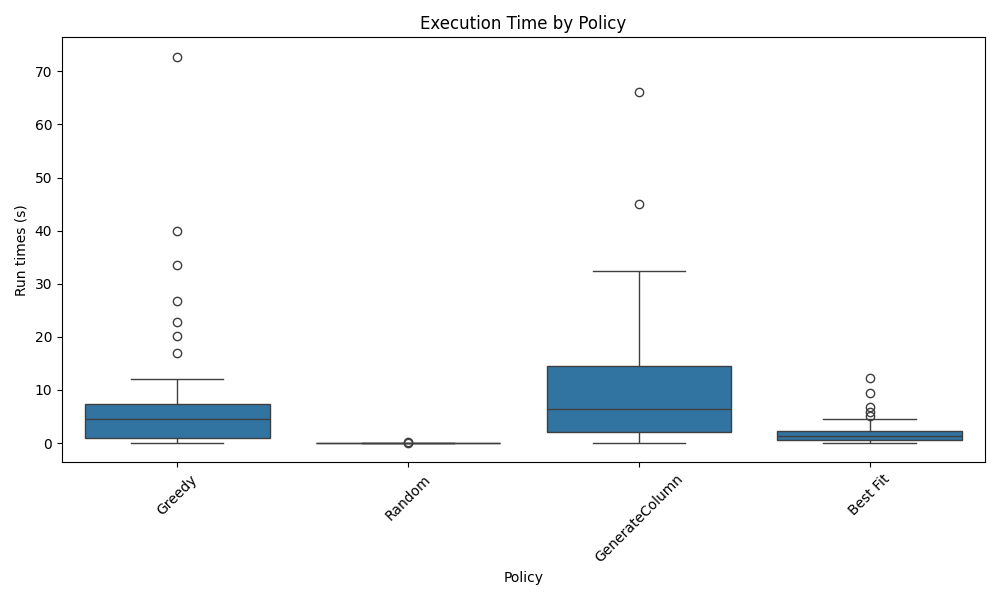
\includegraphics[width=0.5\linewidth]{Images/execution_time_comparison.png}
        \caption{Biểu đồ hộp thể hiện thời gian xử lý trung bình các chính sách sử dụng}
        \label{fig:time}
    \end{figure}
    
    \item \textbf{Lãng phí so với số lượng sản phẩm (Waste vs Number of Products):}
    \begin{itemize}
        \item Biểu đồ phân tán cho thấy chính sách \textit{Random} tạo ra sự gia tăng đáng kể về phần trăm lãng phí khi số lượng sản phẩm tăng, chứng minh đây là chính sách không phù hợp với các tập dữ liệu lớn.
        \item Các chính sách còn lại giữ được mức lãng phí thấp, gần như không bị ảnh hưởng bởi sự gia tăng số lượng sản phẩm. Điều này khẳng định khả năng thích nghi tốt của các chính sách \textit{Greedy}, \textit{GenerateColumn}, và \textit{Best Fit}.
    \end{itemize}
    \begin{figure}[!htp]
        \centering
        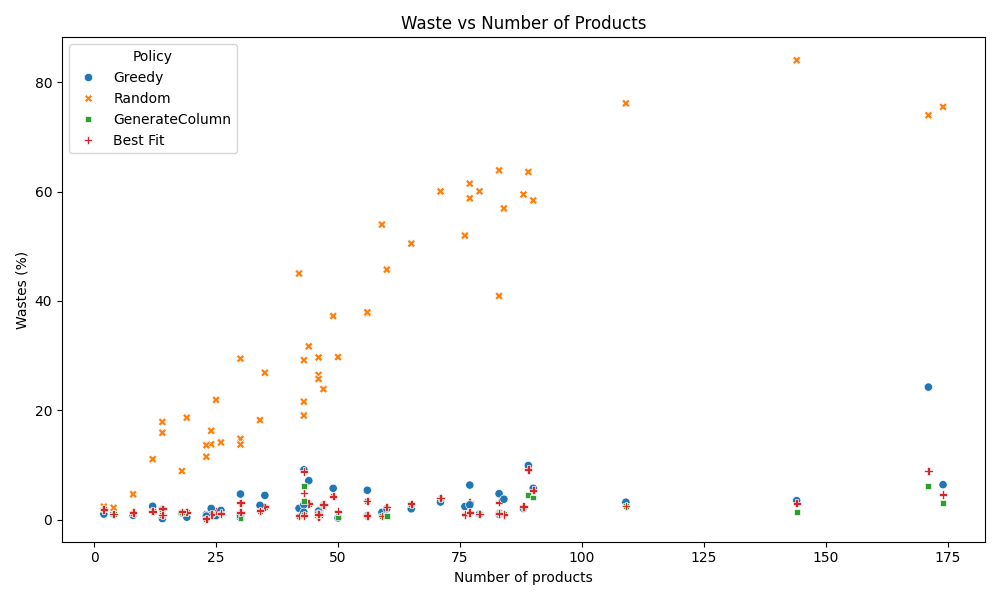
\includegraphics[width=0.5\linewidth]{Images/waste_vs_products.png}
        \caption{Biểu đồ phân tán thể hiện mối quan hệ giữa phần trăm lãng phí và số lượng sản phẩm}
        \label{fig:time}
    \end{figure}
\end{itemize}

\textbf{Kết luận:} Chính sách \textit{Greedy}, \textit{GenerateColumn}, và \textit{Best Fit} đều thể hiện sự tối ưu vượt trội về mặt giảm lãng phí và sử dụng kho lưu trữ. Trong đó, \textit{Best Fit} có ưu thế hơn về cả thời gian thực thi và tối thiểu mức độ lãng phí. Chính sách \textit{Random} tỏ ra không phù hợp cho các ứng dụng thực tế do lãng phí cao và hiệu suất thấp.



\section{Ứng dụng của 2DCSP}
\subsection{Quản lý tài nguyên}

\hspace{0.5cm}Quản lý tài nguyên hiệu quả là một thách thức quan trọng trong nhiều lĩnh vực, đặc biệt là trong các hệ thống máy tính và hoạt động mạng. Vấn đề cắt gọt hai chiều (2D Cutting Stock Problem - 2DCSP), vốn được ứng dụng trong tối ưu hóa vật liệu, mang lại góc nhìn độc đáo khi giải quyết bài toán phân bổ tài nguyên trong các hệ thống này. Bằng cách áp dụng các nguyên lý của 2DCSP vào các ràng buộc tài nguyên đa chiều, bài toán có thể hỗ trợ quản lý tài nguyên như CPU, bộ nhớ, lưu trữ, và băng thông mạng một cách hiệu quả hơn.

\begin{figure}[!htp]
    \centering
    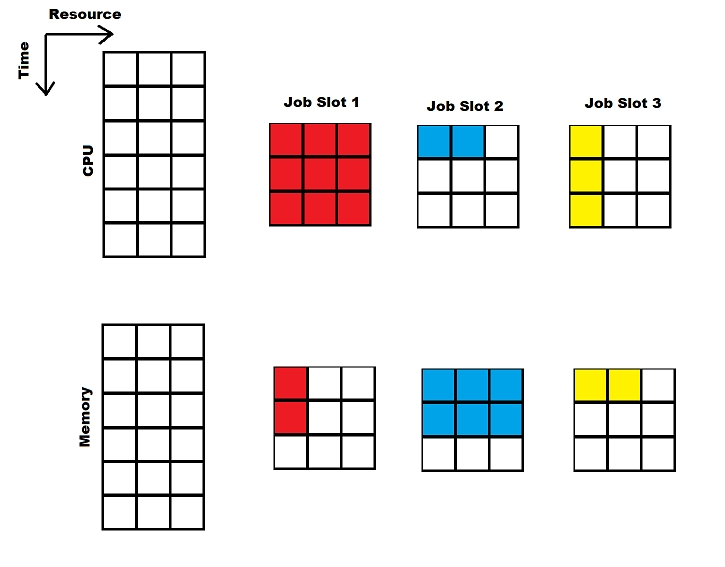
\includegraphics[width=0.5\linewidth]{rm.png}
    \caption{Ví dụ về quản lý tài nguyên với hai loại tài nguyên và ba công việc đang chờ xử lý}
    \label{fig:enter-label}
\end{figure}  

\subsubsection{Thách thức trong quản lý tài nguyên}
\hspace{0.5cm}Quản lý tài nguyên trong các hệ thống máy tính đòi hỏi cân bằng các mục tiêu phức tạp và thường mâu thuẫn, bao gồm tối đa hóa hiệu quả, giảm thiểu độ trễ, và tối ưu hóa việc sử dụng tài nguyên\cite{mao2017resource}. Một số thách thức phổ biến bao gồm:  

\begin{enumerate}[1. ]
    \item \textbf{Sự phức tạp của hệ thống và môi trường động:}
    Các hệ thống hiện đại như cụm máy tính, nền tảng đám mây, và hạ tầng mạng vốn rất phức tạp. Chúng yêu cầu các quyết định được đưa ra trong môi trường thay đổi liên tục, nơi các biến như nhu cầu tài nguyên, nhiễu, và tải hệ thống thay đổi không ngừng.  

    \item \textbf{Ra quyết định trong thời gian thực:}
    Việc phân bổ tài nguyên thường cần được thực hiện trực tuyến, với thời gian tính toán hạn chế và dữ liệu đầu vào có thể không đầy đủ hoặc bị nhiễu. Ví dụ, các nền tảng phát trực tuyến video phải thích ứng với băng thông biến động để đảm bảo phát lại mượt mà.  

    \item \textbf{Ràng buộc đa chiều:}
    Nhu cầu tài nguyên mang tính đa chiều, bao gồm các yếu tố như chu kỳ CPU, không gian bộ nhớ, băng thông I/O, và dung lượng lưu trữ. Phân bổ tài nguyên một cách tối ưu trên các chiều này là một thách thức tổ hợp.  

    \item \textbf{Các chỉ số hiệu suất:}
    Các chỉ số như thời gian hoàn thành công việc, thông lượng hệ thống, và hiệu suất đuôi (tail performance) rất khó để tối ưu hóa đồng thời. Thêm vào đó, mức độ quan trọng của chúng có thể thay đổi tùy theo khối lượng công việc hoặc yêu cầu hệ thống.  
\end{enumerate}  

\subsubsection{Ứng dụng của 2DCSP trong quản lý tài nguyên}  
\hspace{0.5cm}Khung làm việc của 2DCSP giải quyết các thách thức này bằng cách xem việc phân bổ tài nguyên như một bài toán cắt gọt, trong đó mục tiêu là sắp xếp các nhu cầu tài nguyên vào các nguồn lực sẵn có một cách hiệu quả. Quy trình bao gồm các bước sau:  

\begin{enumerate}
    \item \textbf{Mô hình hóa hồ sơ tài nguyên: } 
    Mỗi công việc hoặc tác vụ được biểu diễn dưới dạng một "miếng cắt" hai chiều với các yêu cầu tài nguyên trên nhiều chiều (ví dụ: CPU và bộ nhớ). Các miếng cắt này được sắp xếp vào "nguồn tài nguyên," tương tự như cách phân bổ vật liệu trong bài toán 2DCSP truyền thống.  

    \item \textbf{Mục tiêu tối ưu hóa:} 
    Mục tiêu là giảm thiểu lãng phí tài nguyên trong khi đảm bảo công việc được hoàn thành đúng hạn. Chẳng hạn, trong một kịch bản lập lịch cho cụm máy tính, điều này đồng nghĩa với việc giảm thiểu các khối tài nguyên không sử dụng và đạt được thời gian hoàn thành công việc thấp (job slowdown).  

    \item \textbf{Phương pháp tiếp cận thuật toán: }
    \begin{itemize}
        \item \textbf{Các phương pháp heuristic:} Các thuật toán heuristic truyền thống như chiến lược khớp trước (first-fit) và khớp tốt nhất (best-fit) được điều chỉnh để xử lý các ràng buộc tài nguyên đa chiều.
    \end{itemize}  

    \item \textbf{Mô phỏng và xác nhận:}  
    Các ma trận phân bổ tài nguyên và hồ sơ công việc được sử dụng để mô phỏng kết quả lập lịch. Quy trình này đảm bảo rằng các giải pháp đề xuất đáp ứng các yêu cầu và ràng buộc thực tế.  

    \item \textbf{Triển khai trong các hệ thống thời gian thực:  }
    Các giải pháp 2DCSP nâng cao có thể được triển khai trong các hệ thống quản lý tài nguyên thời gian thực. Ví dụ, trong điện toán đám mây, chúng có thể phân bổ máy ảo vào các máy chủ vật lý, cân bằng khối lượng công việc và giảm thiểu sự phân mảnh.  
\end{enumerate}  

\subsubsection{Lợi ích thực tiễn}  
\hspace{0.5cm}Việc tích hợp 2DCSP vào quản lý tài nguyên mang lại nhiều lợi ích:  

\begin{itemize}
    \item \textbf{Tăng cường sử dụng tài nguyên:} Bằng cách giảm thiểu phân mảnh và lãng phí, hệ thống có thể xử lý nhiều công việc hơn trong cùng một lượng tài nguyên.  
    \item \textbf{Cải thiện hiệu suất hệ thống:} Phân bổ tài nguyên tối ưu giúp giảm thời gian hoàn thành công việc và tuân thủ tốt hơn các thỏa thuận cấp dịch vụ (SLA).  
    \item \textbf{Tính linh hoạt và khả năng mở rộng:} Bản chất thích ứng của các phương pháp 2DCSP cho phép hệ thống xử lý khối lượng công việc đa dạng và phản ứng với các thay đổi động trong nhu cầu.  
    \item \textbf{Giảm chi phí vận hành:} Sử dụng tài nguyên hiệu quả giúp giảm tiêu thụ năng lượng và chi phí phần cứng, mang lại khoản tiết kiệm đáng kể.  
\end{itemize}  


\subsection{Bảng mạch in}

\hspace{0.5cm}Bài toán cắt tấm 2 chiều (2D Cutting Stock Problem - 2DCSP) là một phần cốt lõi trong chiến lược tối ưu hóa của nhiều ngành công nghiệp đòi hỏi sự chính xác và hiệu quả trong việc sử dụng nguyên liệu. Một trong những ứng dụng nổi bật nhất của 2DCSP nằm trong lĩnh vực cắt bảng mạch, một quá trình quan trọng trong sản xuất thiết bị điện tử \cite{ulutas2023effectiveness}. Tính phức tạp và tầm quan trọng của sản xuất bảng mạch đã làm cho 2DCSP trở thành một công cụ không thể thiếu nhằm giải quyết các vấn đề về lãng phí nguyên liệu, hiệu quả vận hành, và tính bền vững với môi trường.

\subsubsection{Tầm quan trọng của tối ưu hóa trong cắt bảng mạch}
\hspace{0.5cm}Bảng mạch đóng vai trò là nền tảng của các thiết bị điện tử hiện đại, đòi hỏi sự chú ý tỉ mỉ trong sản xuất. Quá trình cắt, nhằm định hình các tấm bảng mạch in (PCB) lớn thành các đơn vị nhỏ hơn, đối mặt với nhiều thách thức độc đáo \cite{ulutas2023effectiveness}. Các thách thức này bao gồm:

\begin{enumerate}[1.  ]
    \item Tối đa hóa sử dụng nguyên liệu: Chi phí cao của vật liệu PCB đòi hỏi các chiến lược giảm thiểu lãng phí, đặc biệt trong bối cảnh các thực hành sản xuất bền vững ngày càng được chú trọng.
    \item Đảm bảo độ chính xác về hình học: Mỗi đường cắt phải hoàn toàn phù hợp với các thông số thiết kế của bảng để duy trì tính toàn vẹn của mạch và kết nối.
    \item Xử lý các hình dạng đa dạng và bất thường: Không giống như các hình dạng đơn giản như hình chữ nhật hoặc hình vuông, bảng mạch thường yêu cầu các hình dạng không chuẩn, làm tăng đáng kể độ phức tạp của quá trình tối ưu hóa.
    \item Cân bằng giữa tốc độ và độ chính xác: Với nhu cầu ngày càng tăng về các sản phẩm điện tử, các nhà sản xuất phải tăng quy mô sản xuất trong khi vẫn đảm bảo chất lượng cao.
\end{enumerate}

\subsubsection{Cách 2DCSP giải quyết các thách thức trong cắt bảng mạch}
Phương pháp 2DCSP cung cấp một khung giải pháp mạnh mẽ để xử lý các thách thức này thông qua sự kết hợp giữa mô hình hóa toán học, thiết kế thuật toán, và hiệu quả tính toán. Việc tích hợp 2DCSP vào cắt bảng mạch bao gồm các bước sau:

\begin{figure}[!htp]
    \centering
    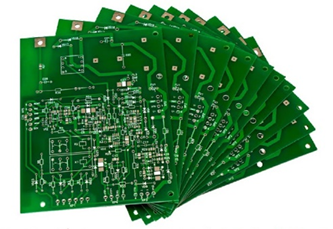
\includegraphics[width=0.3\linewidth]{circuits.png}
    \caption{Mạch điện tử}
    \label{fig:enter-label}
\end{figure}

\begin{enumerate}[1.]
    \item Chuẩn bị dữ liệu và định nghĩa bài toán:
    \begin{itemize}
        \item Các thông số đầu vào như kích thước của vật liệu PCB thô, các hình dạng và kích thước yêu cầu, khả năng của dụng cụ cắt, và các ràng buộc về bố cục được thu thập cẩn thận.
        \item Các thông số này được chuyển đổi thành một biểu diễn chính thức của bài toán 2DCSP, trong đó mục tiêu là giảm thiểu lãng phí trong khi đáp ứng các yêu cầu sản xuất.
    \end{itemize}
    

    \item Các giải pháp thuật toán:
    \begin{itemize}
        \item Một loạt các phương pháp tối ưu hóa có thể được áp dụng, từ các thuật toán chính xác như lập trình tuyến tính và kỹ thuật branch-and-bound đến các phương pháp heuristic và metaheuristic, bao gồm thuật toán di truyền, làm nguội mô phỏng, và tối ưu hóa đàn hạt.
        \item Các thuật toán này đánh giá vô số mẫu cắt tiềm năng, xác định các cấu hình đạt hiệu suất sử dụng nguyên liệu gần tối ưu hoặc tối ưu.
    \end{itemize}


    \item Mô phỏng và cải tiến lặp:
     \begin{itemize}
        \item Khi các giải pháp ban đầu được tạo ra, các mô phỏng sẽ kiểm tra tính khả thi của chúng, xét đến các ràng buộc thực tế như dung sai của máy móc và các khuyết tật vật liệu có thể xảy ra.
        \item Phản hồi từ các mô phỏng được sử dụng để tinh chỉnh các mẫu, đảm bảo đầu ra cuối cùng vừa hiệu quả vừa có thể thực hiện.
    \end{itemize}

    \item Triển khai trong sản xuất:
     \begin{itemize}
        \item Các mẫu đã được xác nhận được tích hợp vào phần mềm của máy cắt, dẫn dắt quá trình cắt vật lý với sự can thiệp tối thiểu của con người.
        \item Các hệ thống tiên tiến tích hợp điều chỉnh thời gian thực, thích ứng động các mẫu trong trường hợp xảy ra các vấn đề bất ngờ, chẳng hạn như sự không đồng nhất của vật liệu.
    \end{itemize}
\end{enumerate}

\subsubsection{Lợi ích đo lường được từ việc áp dụng 2DCSP trong cắt bảng mạch}
\hspace{0.5cm}Việc áp dụng thực tế của 2DCSP đã mang lại những cải thiện mang tính cách mạng trong sản xuất bảng mạch. Các lợi ích đáng chú ý bao gồm:

\begin{figure}[!htp]
    \centering
    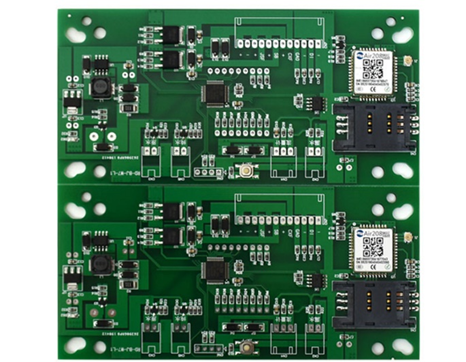
\includegraphics[width=0.5\linewidth]{circuit.png}
    \caption{Thành phần của bảng mạch điện tử}
    \label{fig:enter-label}
\end{figure}

\begin{itemize}
    \item Giảm lãng phí đáng kể: Các nhà sản xuất báo cáo giảm tới 25\% lượng lãng phí nguyên liệu khi sử dụng các mẫu cắt tối ưu so với phương pháp truyền thống.
    \item Tiết kiệm chi phí: Lượng lãng phí giảm dẫn đến chi phí nguyên liệu thấp hơn, trong khi các mẫu cắt hiệu quả cũng giảm thiểu hao mòn máy móc và tiêu thụ năng lượng.
    \item Tăng cường tính linh hoạt: Tính thích ứng của các mô hình 2DCSP cho phép các nhà sản xuất xử lý nhiều loại đơn đặt hàng, từ các thiết kế tiêu chuẩn đến các bố cục được tùy chỉnh cao, mà không làm giảm hiệu quả.
    \item Cải thiện tác động môi trường: Bằng cách giảm thiểu lãng phí và tối ưu hóa việc sử dụng tài nguyên, 2DCSP góp phần vào các thực hành sản xuất bền vững, phù hợp với các nỗ lực toàn cầu nhằm giảm dấu chân carbon của ngành công nghiệp.
\end{itemize}

\section{Kết luận}
\subsection{Hướng nghiên cứu trong tương lai}

\hspace{0.5cm}Bài toán cắt tấm hai chiều (2DCSP) đại diện cho một thách thức thú vị và phức tạp trong lĩnh vực tối ưu hóa, với các ứng dụng cả về lý thuyết và thực tiễn. Là một lĩnh vực nghiên cứu quan trọng, bài toán này tiếp tục truyền cảm hứng cho việc phát triển các thuật toán và phương pháp luận đổi mới. Trong tương lai, chúng tôi dự định khám phá các kỹ thuật tối ưu hóa đa dạng nhằm cải thiện hiệu quả và khả năng mở rộng của các giải pháp cho 2DCSP. Điều này không chỉ bao gồm các phương pháp truyền thống như thuật toán metaheuristic và thuật toán chính xác mà còn cả các cách tiếp cận tiên tiến tích hợp trí tuệ nhân tạo.

Một trong những hướng đi hứa hẹn nhất mà chúng tôi hướng tới là áp dụng Học Máy, đặc biệt là Học Tăng Cường (Reinforcement Learning), để giải quyết 2DCSP. Nhờ vào khả năng của Học Tăng Cường trong việc ra quyết định tuần tự trong các môi trường động, chúng ta có thể khám phá những chiến lược mới cho tối ưu hóa thời gian thực và giải quyết vấn đề một cách thích ứng \cite{RL}. Ngoài ra, việc tích hợp các mô hình học có giám sát và không giám sát có thể cung cấp góc nhìn mới về nhận dạng mẫu và dự đoán trong khuôn khổ 2DCSP.

Bên cạnh việc cải tiến thuật toán, chúng tôi nhận thấy cơ hội đáng kể trong việc áp dụng các giải pháp 2DCSP vào nhiều ngành công nghiệp mới nổi và các lĩnh vực liên ngành. Điều này bao gồm quản lý tài nguyên \cite{mao2017resource}, nơi sử dụng nguyên liệu hiệu quả là rất quan trọng; điện toán hiệu năng cao (HPC) \cite{le2023irls}, đòi hỏi sự tối ưu hóa trong việc lập lịch nhiệm vụ và phân bổ tài nguyên; và thiết kế vi mạch, nơi tối ưu hóa bố cục có thể giảm chi phí và cải thiện hiệu suất. Hơn nữa, các nguyên tắc của 2DCSP có thể truyền cảm hứng cho những cách tiếp cận đổi mới trong logistics, quản lý kho bãi và sản xuất phụ gia.

Việc mở rộng phạm vi nghiên cứu 2DCSP cũng liên quan đến việc giải quyết các hạn chế và mở rộng các giải pháp để xử lý các kịch bản thực tế ngày càng phức tạp. Điều này đòi hỏi việc phát triển các thuật toán mạnh mẽ có khả năng đáp ứng các ràng buộc như hình dạng không đều, đặc tính vật liệu khác nhau và điều kiện tồn kho động. Các hợp tác giữa giới học thuật và ngành công nghiệp có thể thúc đẩy nhanh việc chuyển giao các tiến bộ lý thuyết thành các ứng dụng thực tiễn.

Tóm lại, 2DCSP vẫn là một lĩnh vực giàu tiềm năng cho sự đổi mới và khám phá. Bằng cách tiếp cận các kỹ thuật tiên tiến và khám phá các ứng dụng trong nhiều lĩnh vực khác nhau, chúng tôi hy vọng đóng góp vào sự hiểu biết học thuật về vấn đề này và tác động chuyển đổi của nó đối với các ngành công nghiệp trên toàn cầu.

\subsection{Lời kết}

Bài toán cắt tấm hai chiều (2DCSP) là một thách thức quan trọng nằm ở giao điểm giữa tối ưu hóa toán học và hiệu quả công nghiệp. Thông qua nghiên cứu này, chúng tôi đã minh chứng tính linh hoạt và hiệu quả của việc kết hợp mô hình toán học chặt chẽ, các chiến lược heuristic, và các phương pháp tiếp cận học máy tiên tiến để giải quyết bài toán phức tạp này. Việc tích hợp nền tảng lý thuyết với các ứng dụng thực tiễn nhấn mạnh tiềm năng của 2DCSP trong việc tối ưu hóa sử dụng vật liệu, giảm lãng phí và nâng cao hiệu quả vận hành trong nhiều ngành công nghiệp khác nhau. 

Mặc dù các thuật toán và phương pháp được trình bày đã chứng minh hiệu quả trong việc giải quyết nhiều kịch bản thực tế, chẳng hạn như quản lý tài nguyên và cắt bảng mạch in, chúng cũng phản ánh tính chất không ngừng phát triển của các bài toán tối ưu hóa trước sự gia tăng độ phức tạp và các ràng buộc động. Trong tương lai, việc khám phá các phương pháp tiếp cận dựa trên trí tuệ nhân tạo và các ứng dụng liên ngành mở ra những hướng đi mới đầy thú vị, hứa hẹn những giải pháp không chỉ hiệu quả mà còn thích ứng với các thách thức mới. Cuối cùng, nghiên cứu này phản ánh cam kết của chúng tôi trong việc thúc đẩy nghiên cứu tối ưu hóa đồng thời thu hẹp khoảng cách giữa lý thuyết và thực tiễn, đóng góp những hiểu biết có ý nghĩa và các giải pháp có tác động đến cả học thuật và ngành công nghiệp.


% for testing

% REFERENCES
\pagebreak
\nocite{*}
\printbibliography[
heading=bibintoc,
title={Tài liệu tham khảo}
]
\end{document}

